The third category of inputs for \mocasin is \texttt{sdf3}, which uses the \ac{\SDFFF} framework~\cite{sdf3}.
This framework is based on \ac{TGFF}, adapted to the \ac{SDF} model of computation.
We will discuss \ac{SDF} more in detail in Chapter~\ref{chap:mocs}.
However, for the purposes of benchmarking as discussed here, both \ac{SDF} and task graphs can be considered as special cases of \ac{KPN}.
The random graph generation of the \ac{\SDFFF} framework allows multiple configurations on the types of graphs it generates, controlling the number of actors (processes) as well as the degree of connectivity in the graph, firing rates and execution times of the actors, or if the graph is acycilic.

Random benchmark generation has two main advantages over using fixed benchmarks. The first advantage is the amount of benchmarks, which is virtually unlimited with a random generation approach.
The second advantage is the control over the properties of the benchmarks.
Using \ac{\SDFFF} we can consider precisely what effect the properties of the graph have on the algorithms (e.g. its size, or connectivity), by generating benchmarks which have the desired parameters for the independent variable we are investigating.
The main disadvantage is obvious: random benchmarks are not as realistic as actual benchmarks.
It is not clear if we will find a graph like the one generated by \ac{\SDFFF} in a real-life application.

Since we have both the \ac{CPN} and the \ac{E3S} benchmarks, we will focus our evaluation on those.
Instead of discussing the graph generation in \ac{SDFFF}, we will discuss random benchmark generation from a different type of graph, \emph{level graphs}\index{level graph}\cite{goens_multiprog18}.
The main difference is that for the use-case for level graphs in~\cite{goens_multiprog18} we \textbf{do not} have better, realistic benchmark we can use instead.

The context for benchmark generation we will discuss here is in microservice-oriented architectures.
In large internet companies like Facebook or Twitter, the infrastructure of the architecture consists of multiple micro-services that depend on each other.
A crucial factor for optimal performance is the amount of \ac{I/O} calls these microservices make.
We will discuss the use case more in-depth in Chapter~\ref{chap:programming_languages}. 
In this section we will only focus on the benchmark generation.

The microservice-based infrastructures from large companies like Facebook or Twitter are the \acf{IP} of these companies and not in the public domain.
If we want to improve and compare a method for optimizing \ac{I/O} in Facebook's spam-fighting service~\cite{marlow2014haxl}, we cannot use a large representative benchmark sample from Facebook to test against their method.
Instead, we observe the general structure of the programs in their work and device a methodology for generating random benchmarks, with a method we call level graphs~\cite{goens_multiprog18}.

Figure~\ref{fig:level_graph} shows an example of a level graph. 

TODO: describe graph construction and briefly outline code generation.

\begin{figure*}[th]
	\centering
	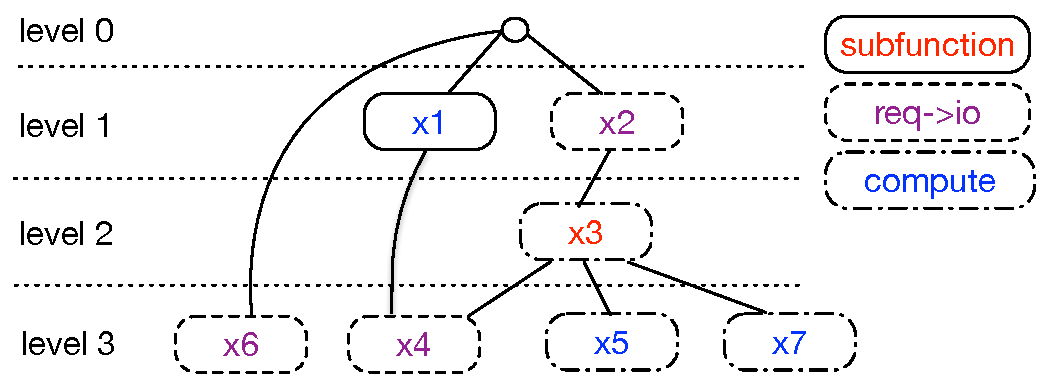
\includegraphics[width=\textwidth]{figures/level-graph.pdf}
	\caption{An example of a Level Graph. Reproduced from Figure~1 of \cite{goens_multiprog18}.}
	\label{fig:histograms}
\end{figure*}